\begin{figure}[ht]
	\begin{center}
	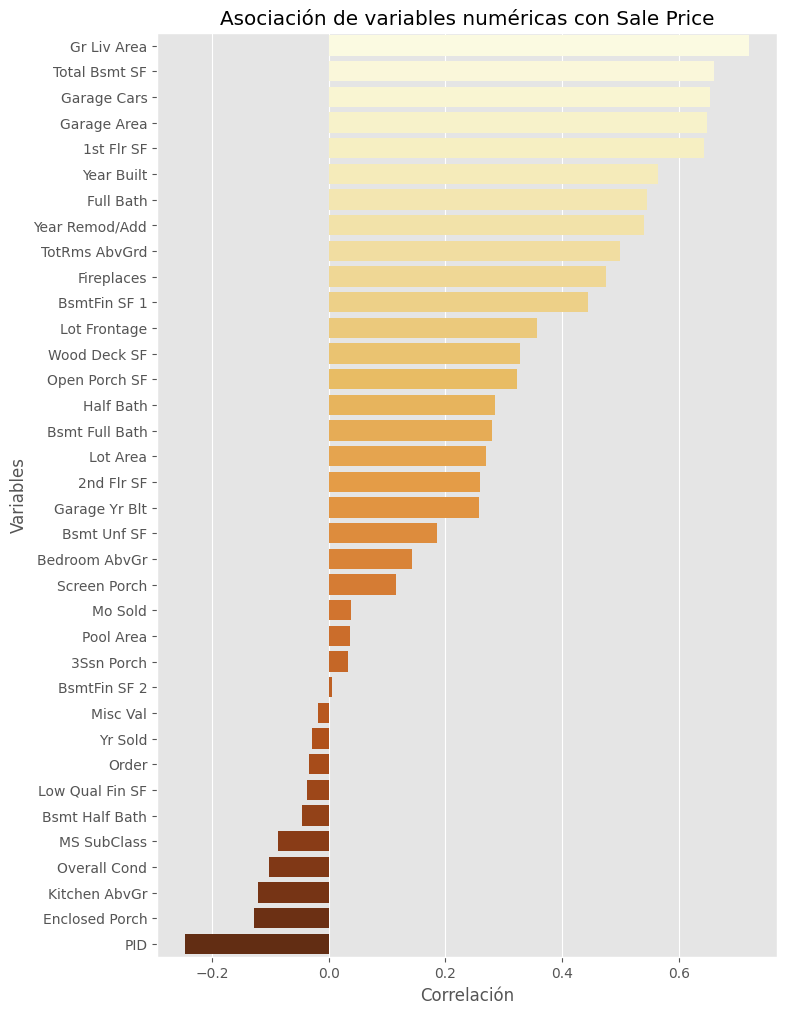
\includegraphics[width=0.5\textwidth]{figures/Asociacion de Variables Numericas con Sale Price.png}
	\caption[Asociación de variables numéricas con \textit{SalePrice}]{Asociación de variables numéricas con \textit{SalePrice}.}
	\label{fig:grafico numericas y SalePrice}
	\end{center}
\end{figure}

\begin{figure}[ht]
	\begin{center}
	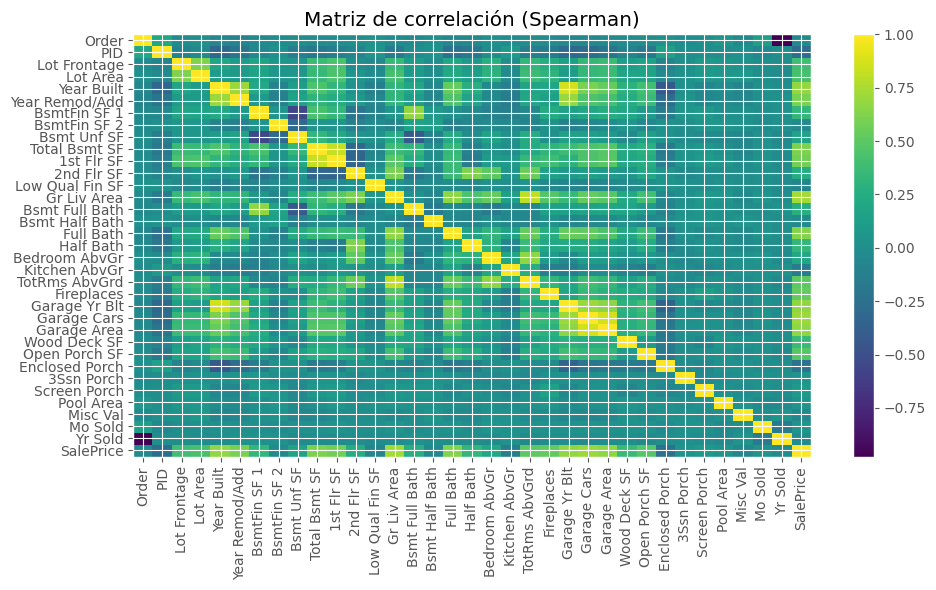
\includegraphics[width=0.5\textwidth]{figures/Matriz de Correlación Spearman.png}
	\caption[Matriz de correlación de \textit{Spearman} de variables cuantitativas]{Matriz de correlación de \textit{Spearman} de variables cuantitativas.}
	\label{fig:graficocuantitativospear}
	\end{center}
\end{figure}


\begin{figure}[ht]
	\begin{center}
	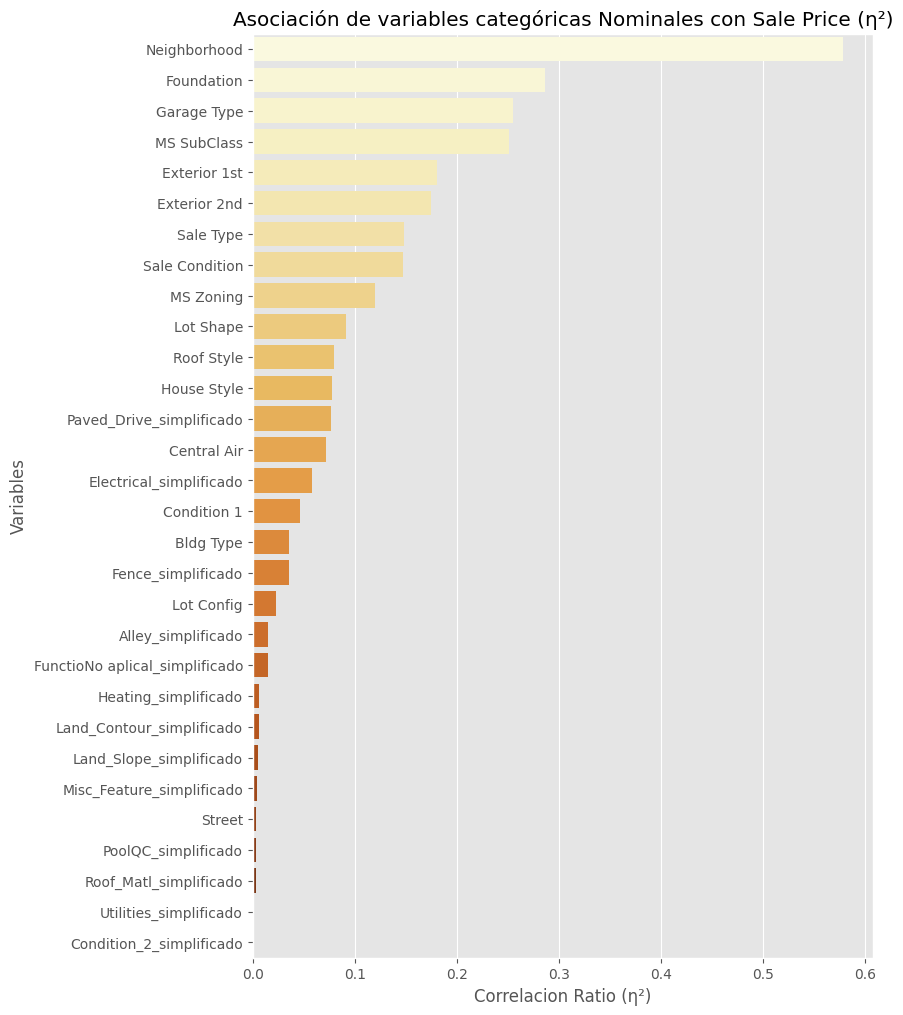
\includegraphics[width=0.5\textwidth]{figures/Asociación de variables categóricas nominales con Sale Price.png}
	\caption[Asociación de variables categóricas nominales con \textit{Sale Price}.]{Asociación de variables categóricas nominales con \textit{Sale Price}.}
	\label{fig:asociación categórica nominal con SP}
	\end{center}
\end{figure}

\begin{figure}[ht]
	\begin{center}
	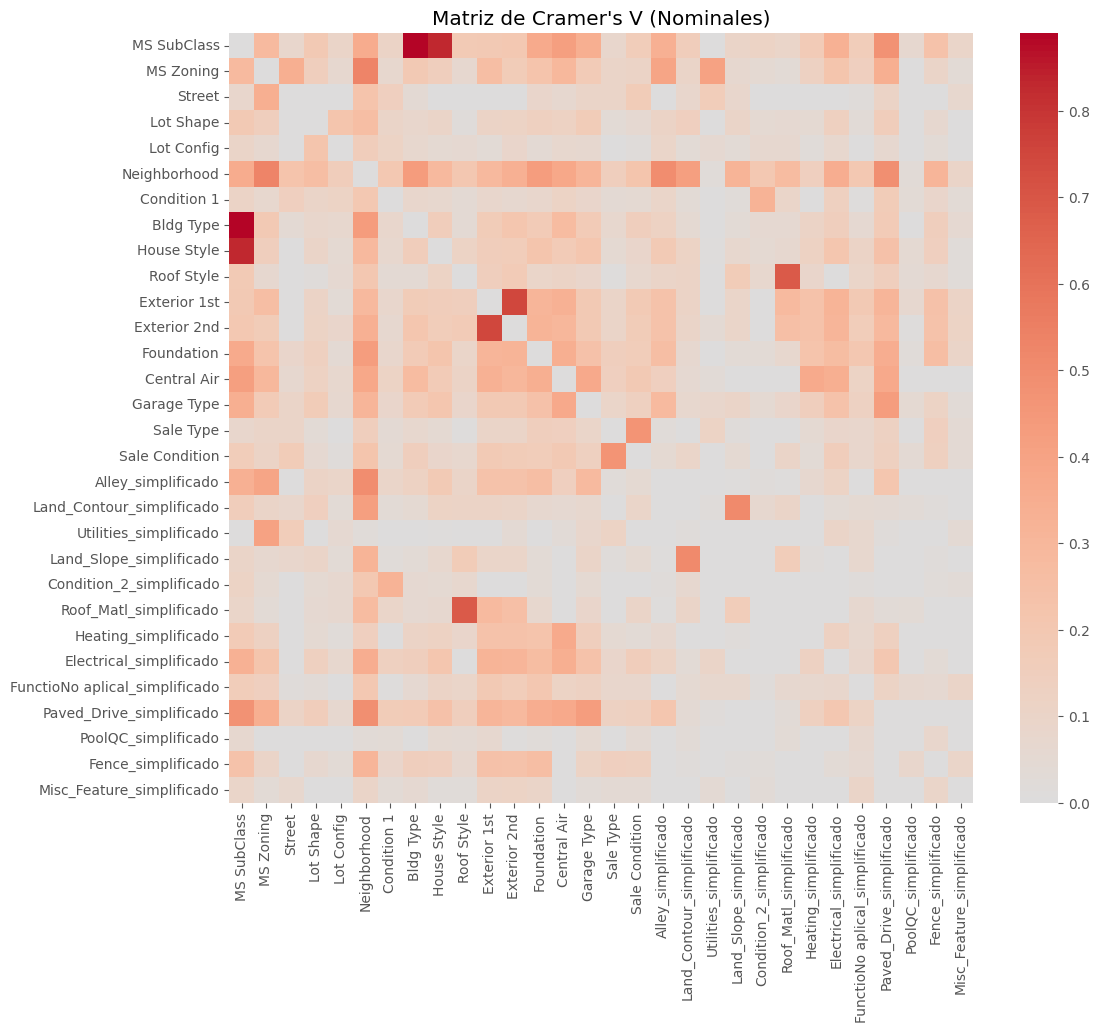
\includegraphics[width=0.5\textwidth]{figures/Matriz Cramer.png}
	\caption[Matriz de Cramer’s V de variables categóricas nominales]{Matriz de Cramer’s V de variables categóricas nominales.}
	\label{fig:cramerV nominales}
	\end{center}
\end{figure}
\clearpage
\begin{figure}[H]
	\begin{center}
	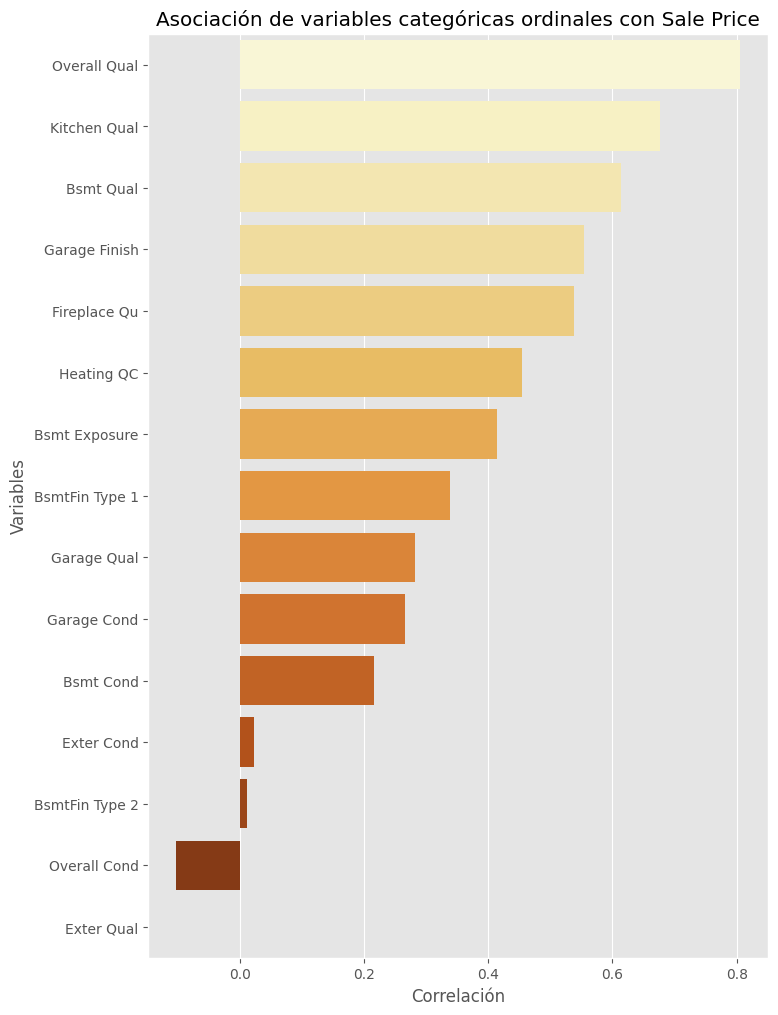
\includegraphics[width=0.5\textwidth]{figures/Asociación de variables categóricas ordinales con Sale Price.png}
	\caption[Asociación de variables categóricas Ordinales con \textit{Sale Price}.]{Asociación de variables categóricas Ordinales con \textit{Sale Price}.}
	\label{fig:precio con categorica ordinal}
	\end{center}
\end{figure}

\begin{figure}[ht]
	\begin{center}
	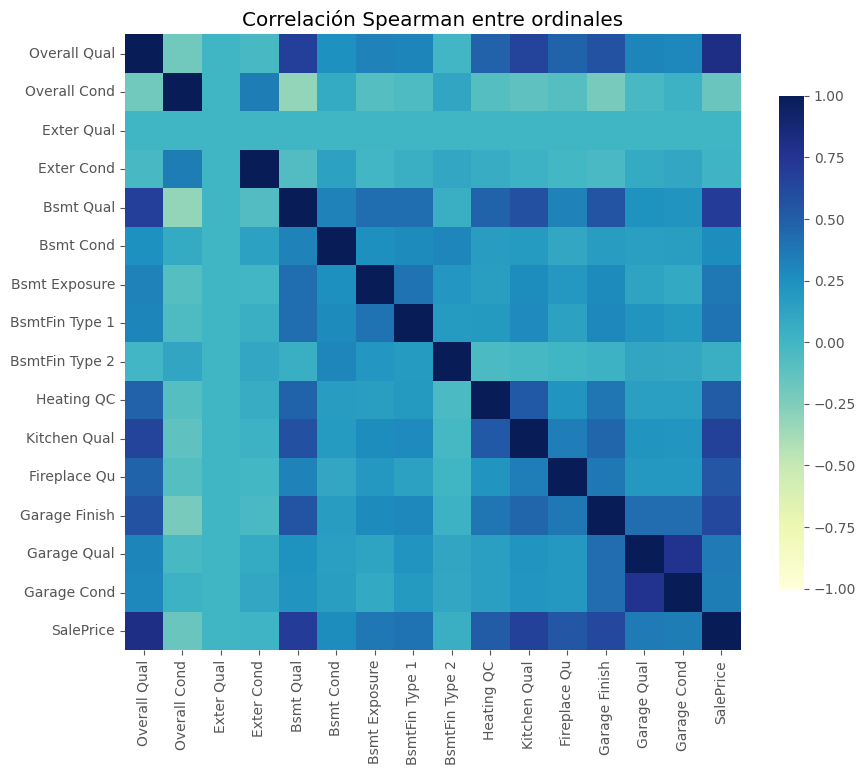
\includegraphics[width=0.5\textwidth]{figures/Correlación Spearman entre ordinales.png}
	\caption[Matriz de correlación de  Spearman de variables categóricas ordinales codificadas]{Matriz de correlación de Spearman de variables categóricas ordinales codificadas.}
	\label{fig:spearman categórica ordinal}
	\end{center}
\end{figure}

\begin{figure}[ht]
	\begin{center}
	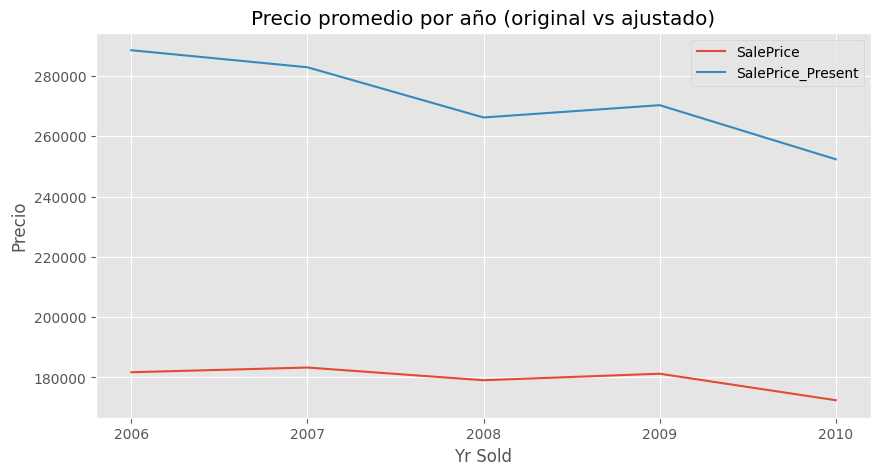
\includegraphics[width=0.5\textwidth]{figures/Ajuste IPC.png}
	\caption[Precio original vs ajustado]{Gráfico promedio de \textit{SalePrice} por año, ajustado por IPC al precio presente}
	\label{fig:Preciooriginalvsajustado}
	\end{center}
\end{figure}

\begin{figure}[ht]
	\begin{center}
	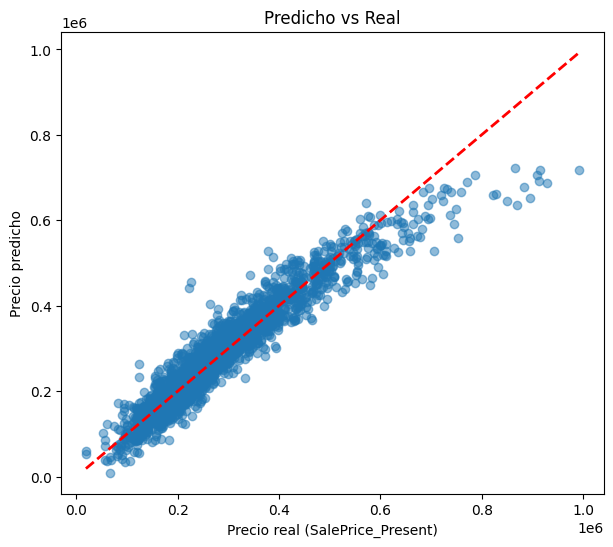
\includegraphics[width=0.5\textwidth]{figures/Regresion Normal.png}
	\caption[Regresión Lineal \textit{SalePrice\_Present}]{Regresión Lineal \textit{SalePrice\_Present}}
	\label{fig:regresioninicial}
	\end{center}
\end{figure}

\begin{figure}[ht]
	\begin{center}
	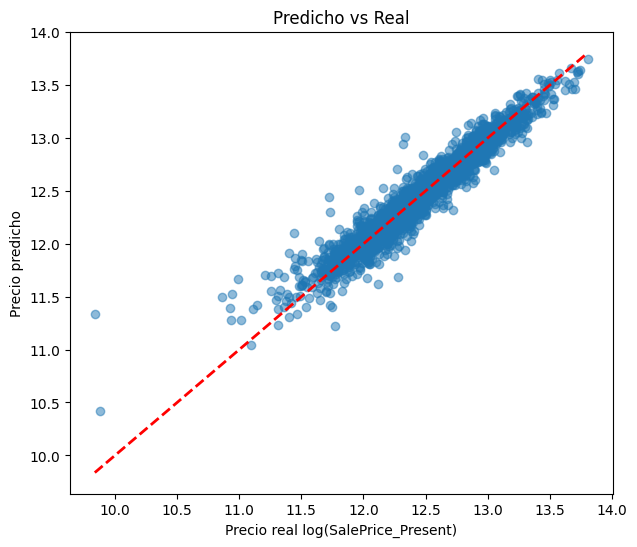
\includegraphics[width=0.5\textwidth]{figures/Regresion Log(Sale Price).png}
	\caption[Regresión Lineal \textit{log(SalePrice\_present)}.]{Regresión Lineal \textit{log(SalePrice\_present)}.}
	\label{fig:grafico logSalePrice con precio}
	\end{center}
\end{figure}

\begin{figure}[ht]
	\begin{center}
	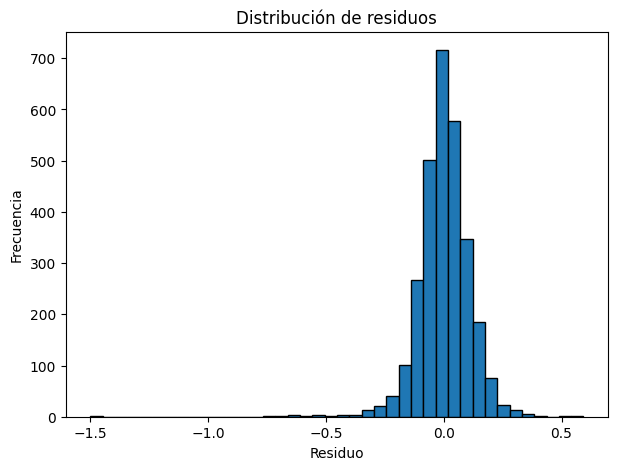
\includegraphics[width=0.5\textwidth]{figures/Residuos Regresión Log Sale Price .png}
	\caption[Distribución de residuos al aplicar \textit{log(SalePrice\_Present)}]{Distribución de residuos al aplicar \textit{log(SalePrice\_Present)}}
	\label{fig:distribucionderesiduoscon log}
	\end{center}
\end{figure}

\begin{figure}[ht]
    \centering
    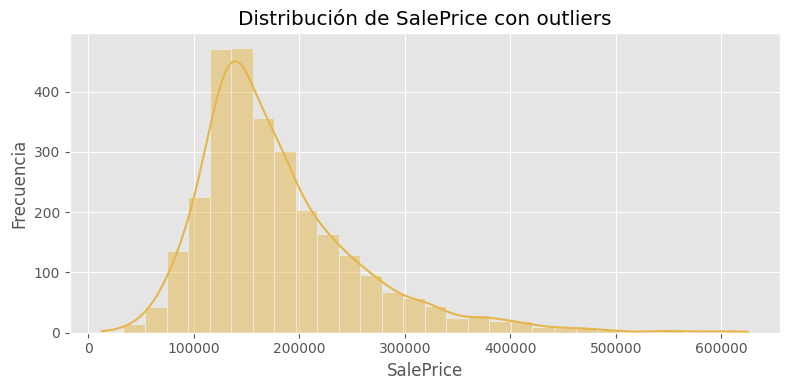
\includegraphics[width=0.5\textwidth]{figures/Distribución de Sale Price con Outliers.png}
    \caption[Distribución SalePrice]{Distribución de \textit{SalePrice} con \textit{outliers.}}
    \label{fig:residuos con outliers}
\end{figure}

\begin{figure}[ht]
	\begin{center}
	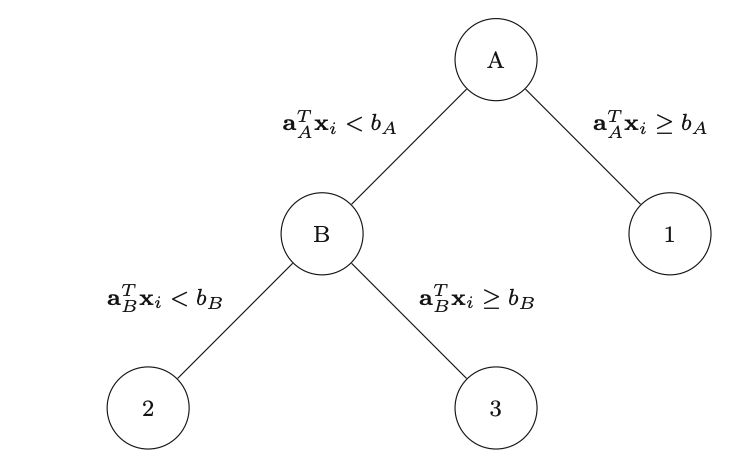
\includegraphics[width=0.5\textwidth]{figures/arboldecision.png}
	\caption[Árbol de decisión con dos nodos de partición y tres nodos hoja.]{Árbol de decisión con dos nodos de partición y tres nodos hoja. \cite{Bertsimas2017}}
	\label{fig:arboldecision}
	\end{center}
\end{figure}

\begin{figure}[ht]
\centering
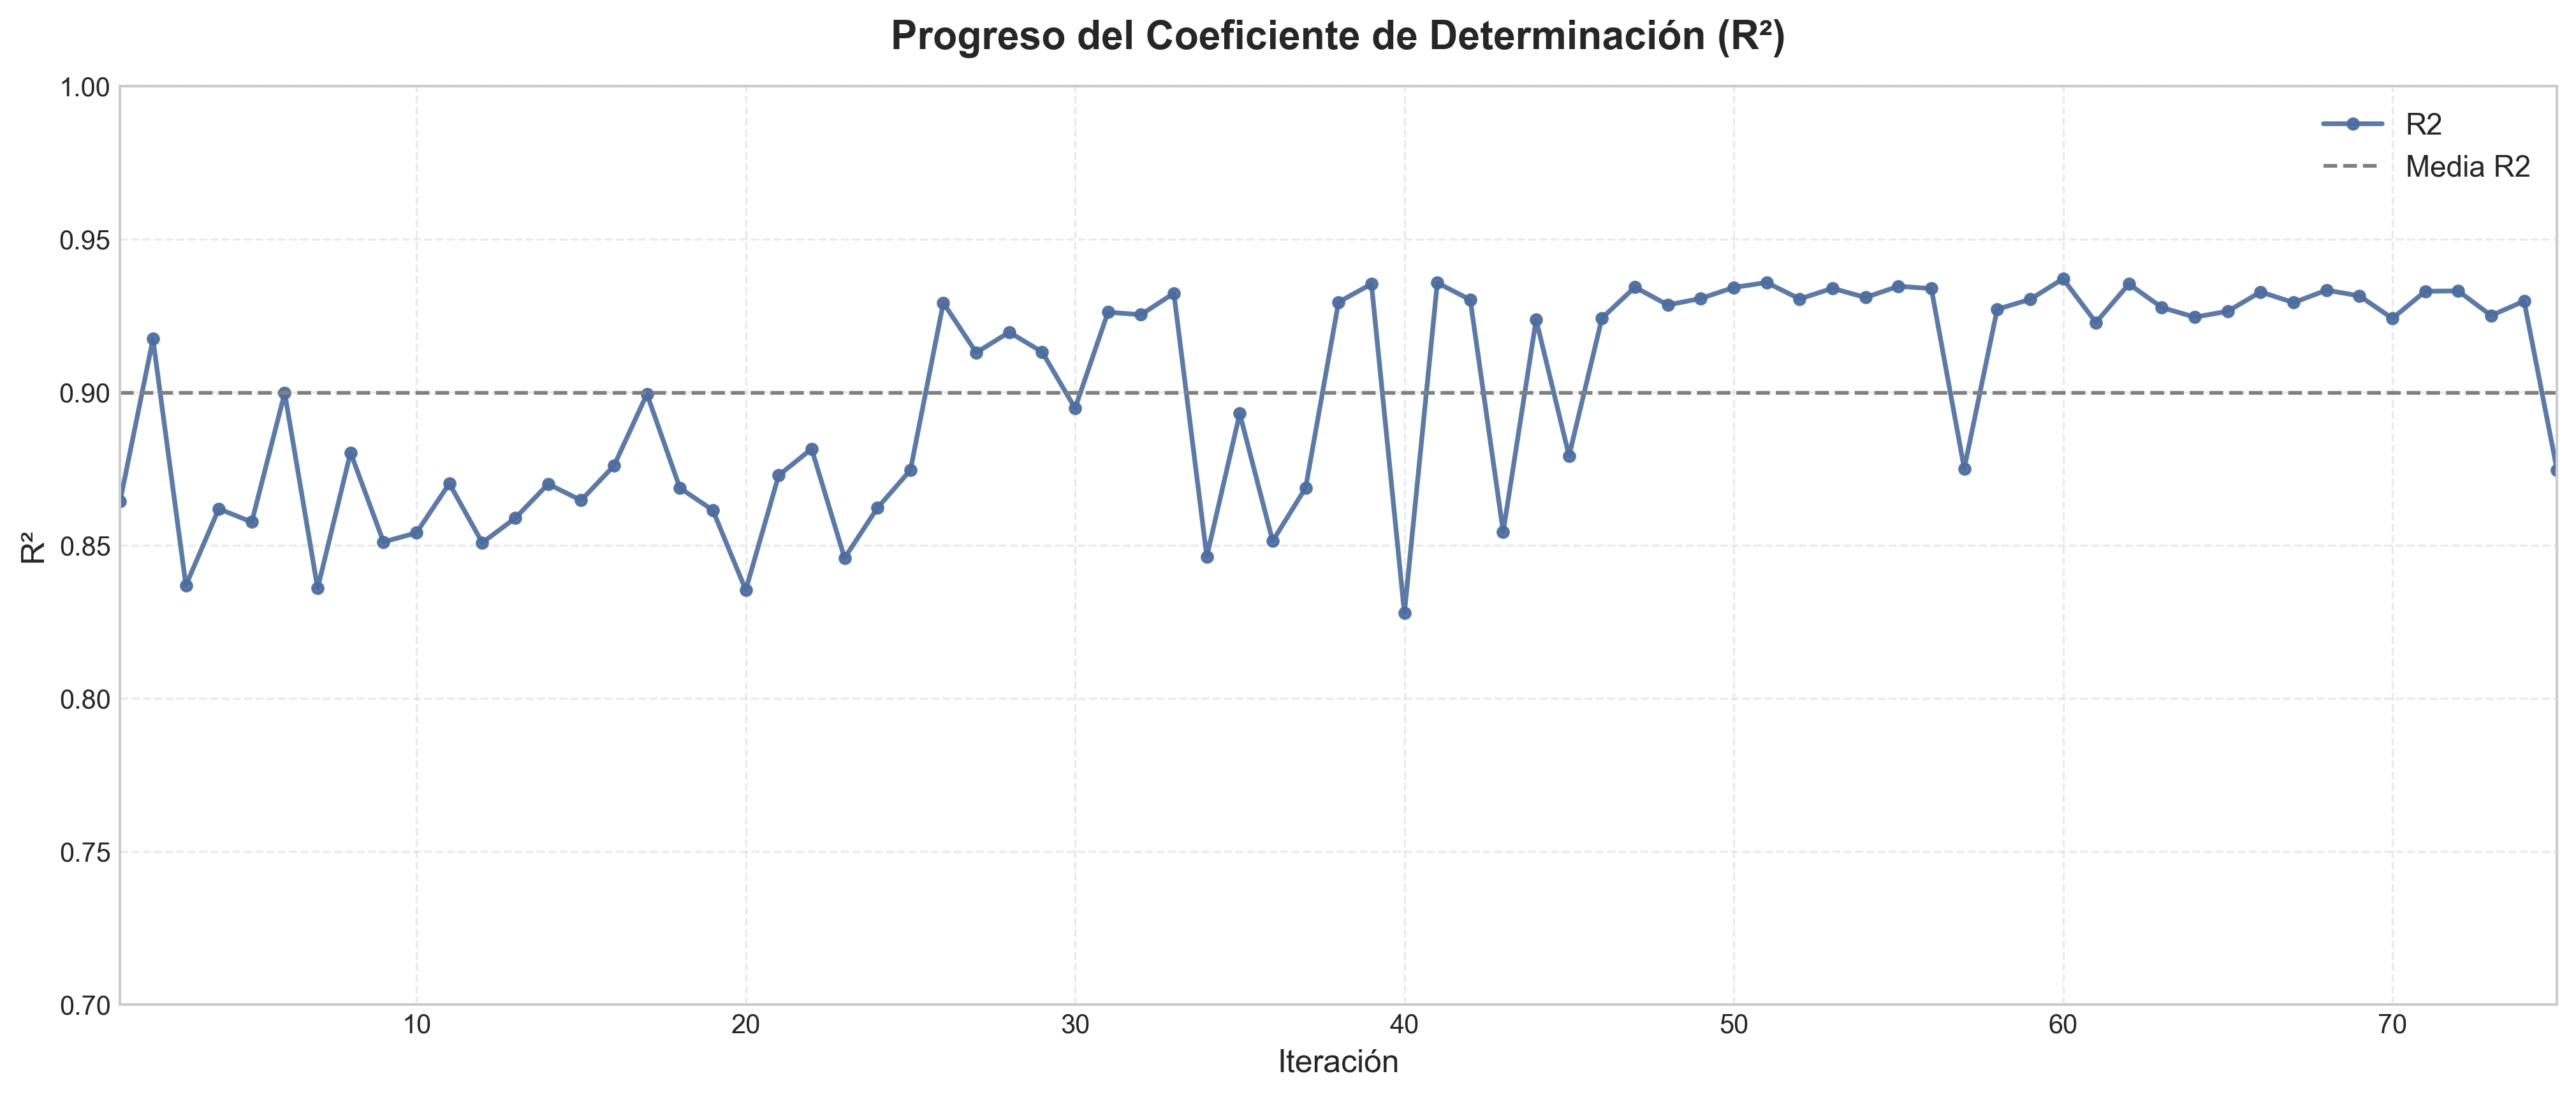
\includegraphics[width=0.6\textwidth]{figures/r2_iter_75.png}
\caption{Evoluci\'on $R^{2}$ con respecto al tiempo}
\label{fig:r2_iter}
\end{figure}

\begin{figure}[ht]
\centering
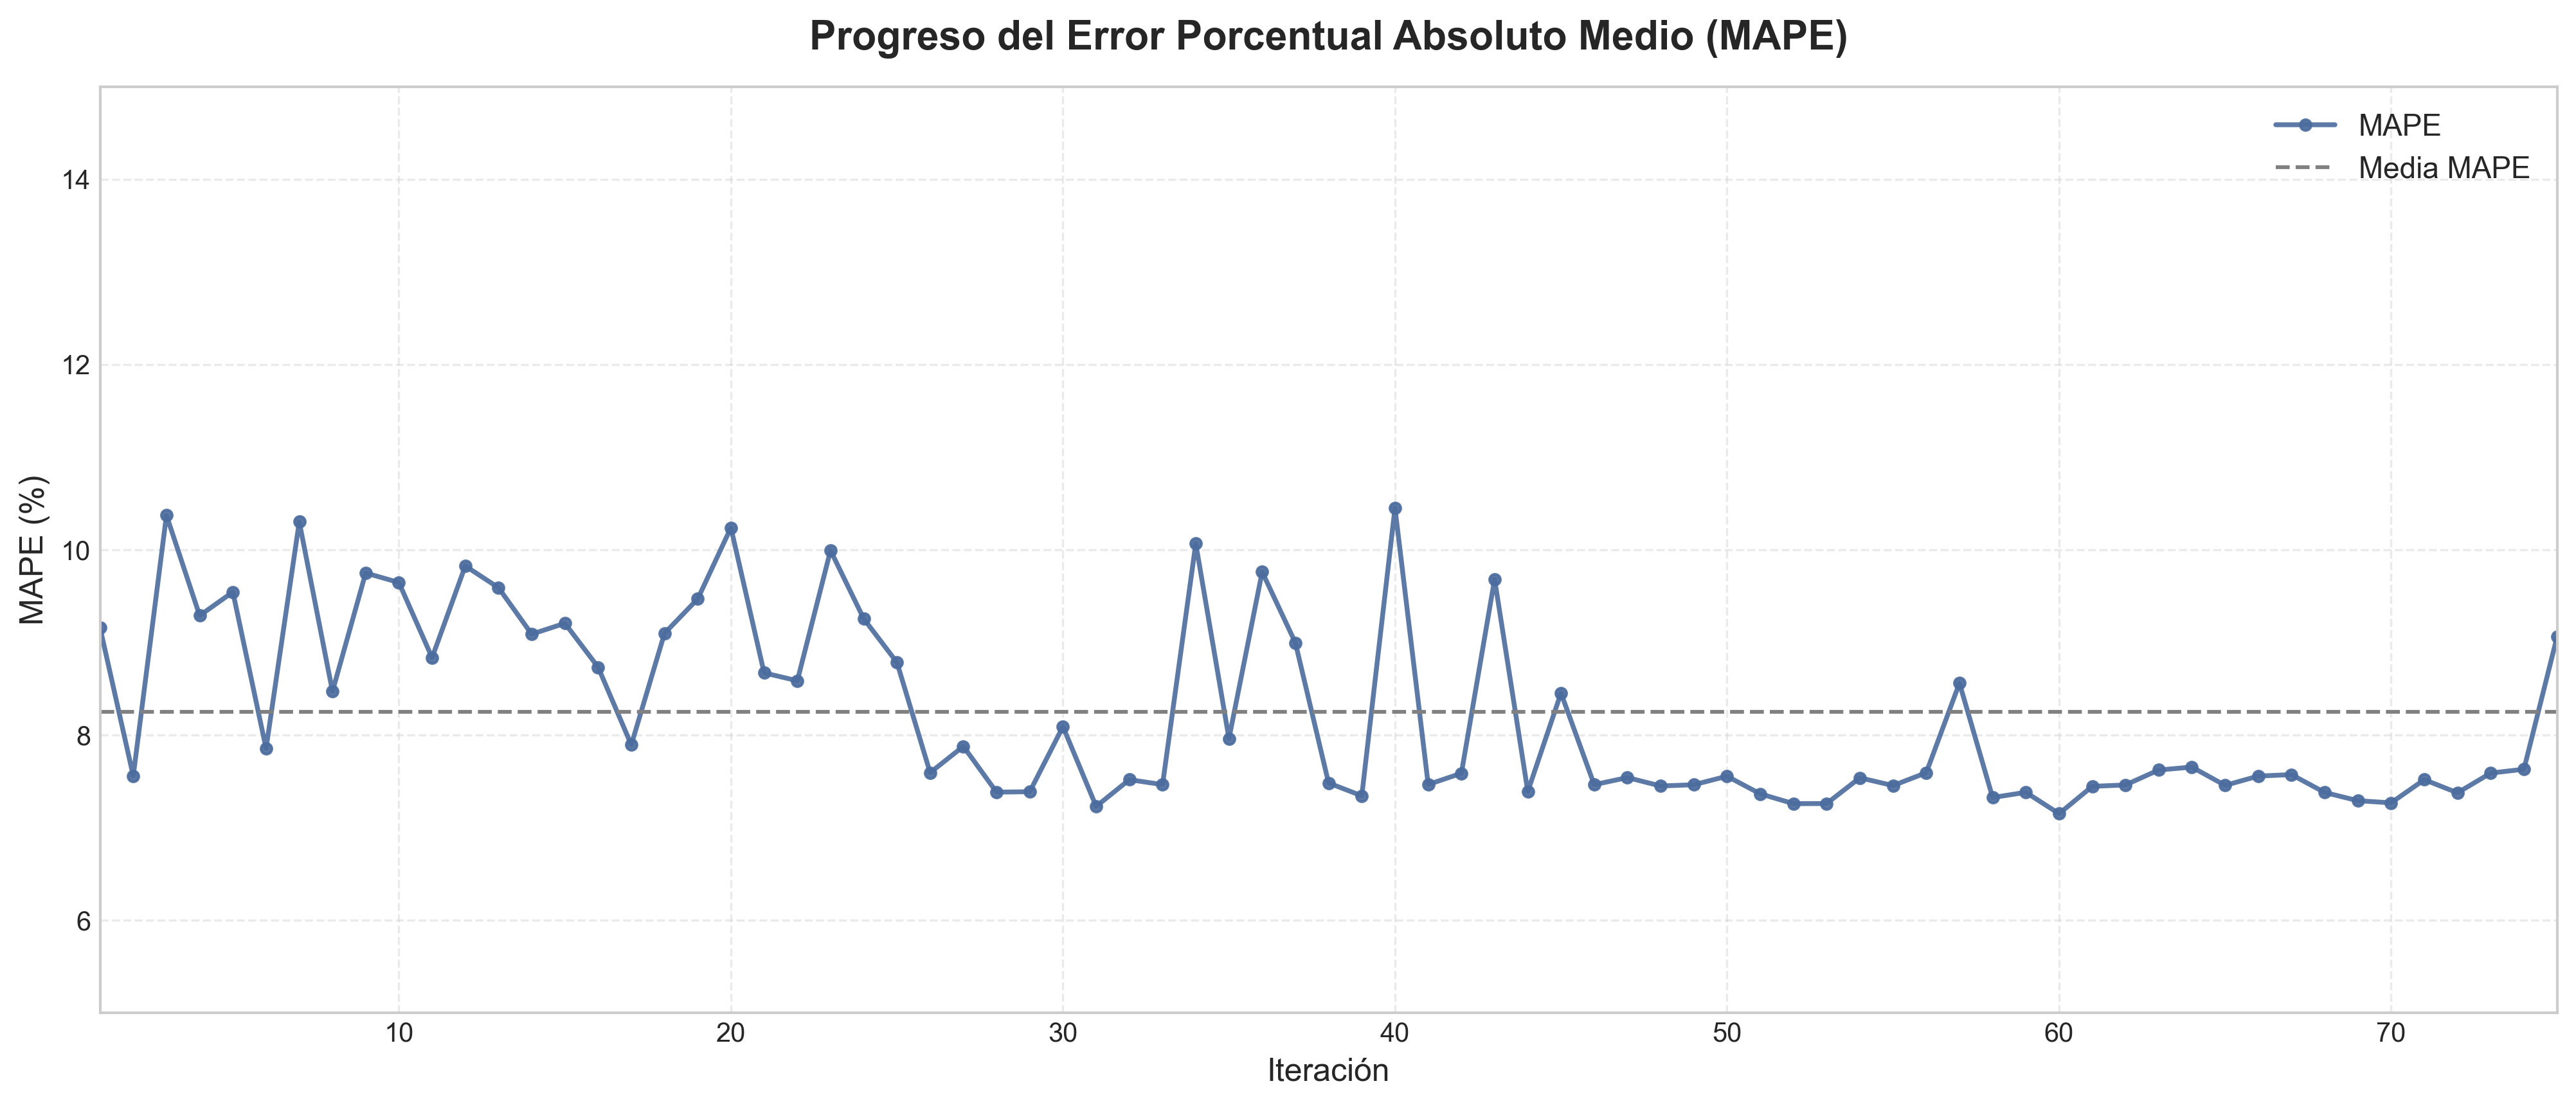
\includegraphics[width=0.6\textwidth]{figures/mape_iter_75.png}
\caption{Evoluci\'on MAPE con respecto al tiempo}
\label{fig:mape_iter}
\end{figure}

\begin{figure}[ht]
\centering
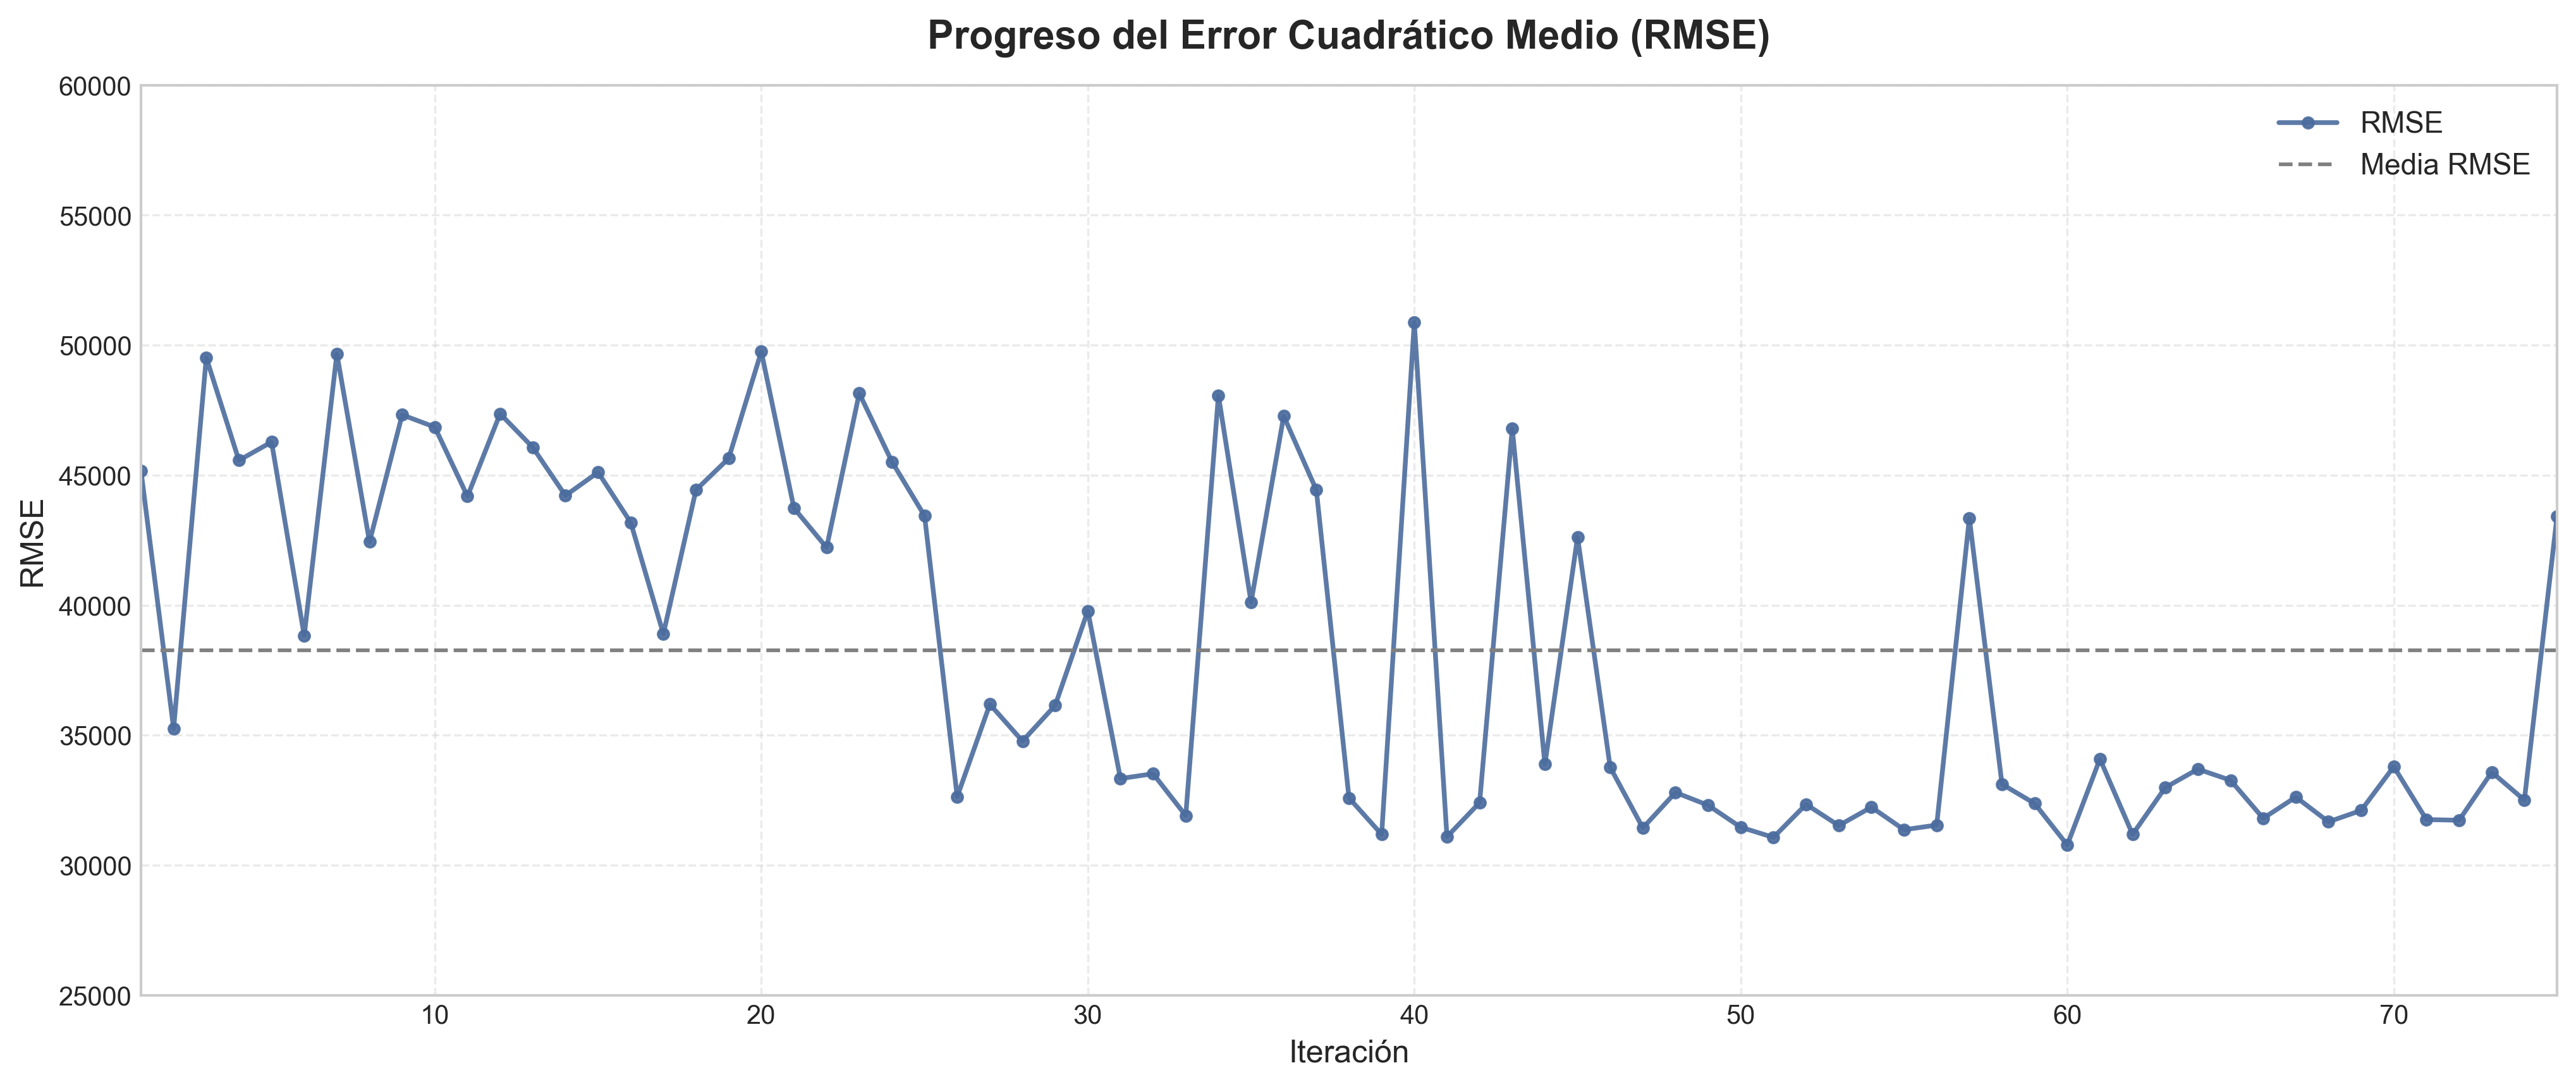
\includegraphics[width=0.6\textwidth]{figures/rmse_iter_75.png}
\caption{Evoluci\'on RMSE con respecto al tiempo}
\label{fig:rmse_iter}
\end{figure}

\begin{figure}[ht]
\centering
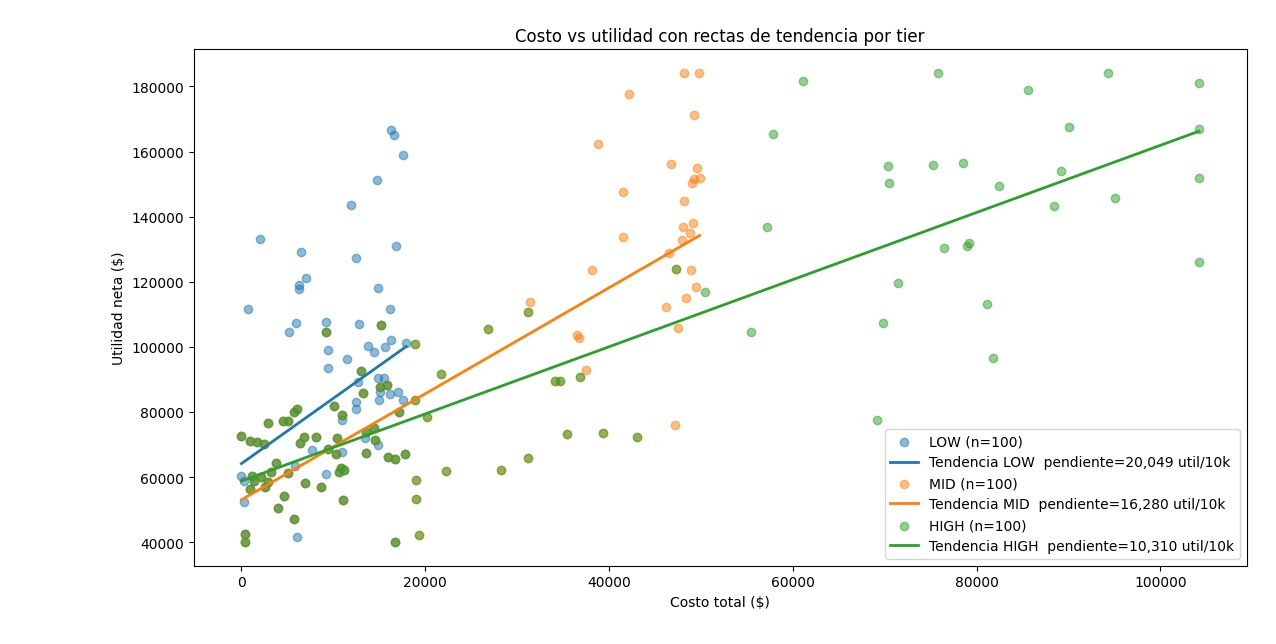
\includegraphics[width=0.6\textwidth]{figures/utilidad vs costo.jpg}
\caption{Diagrama Costo vs Utilidad con rectas de tendencia para los distintos presupuestos. Las pendientes representan la utilidad por cada 10k más de presupuesto.}
\label{fig:costo vs utilidad}
\end{figure}

\begin{figure}[ht]
	\begin{center}
	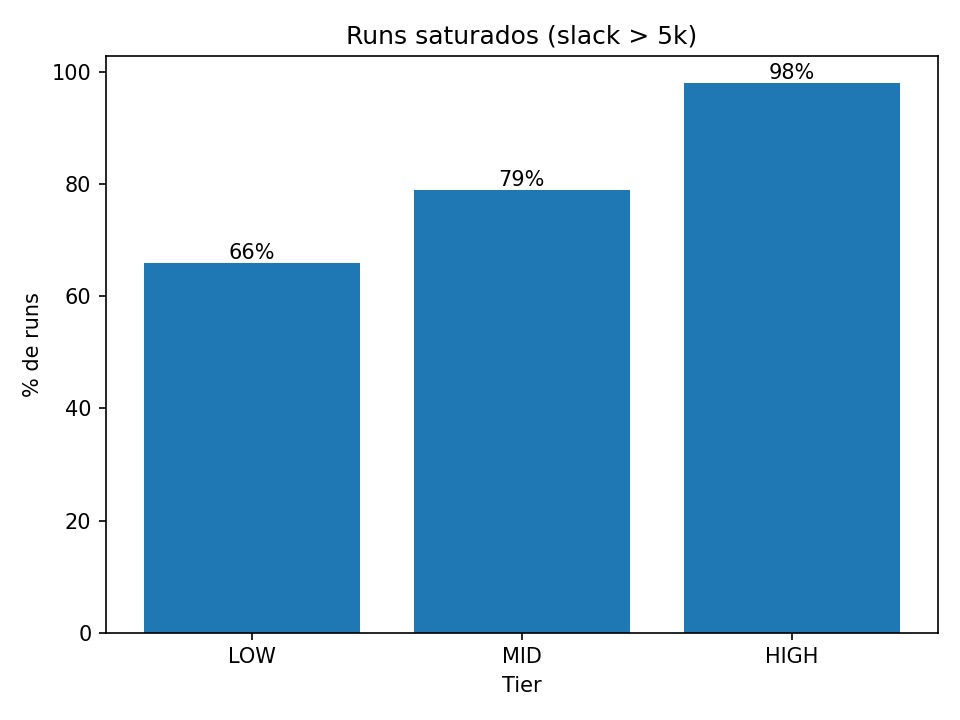
\includegraphics[width=0.5\textwidth]{figures/slacks saturados.jpg}
	\caption[]{Gráfico que muestra porcentaje de casas que les sobra más de 5K luego de la remodelación}
	\label{fig:slackssaturados}
	\end{center}
\end{figure}

\begin{figure}[ht]
	\begin{center}
	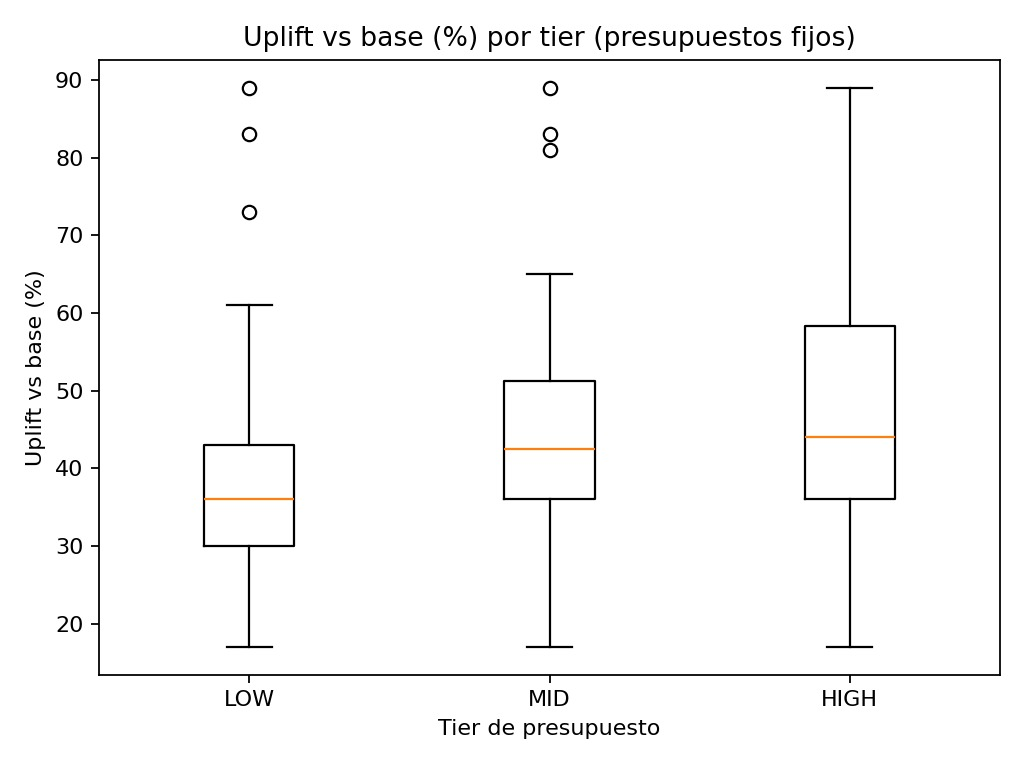
\includegraphics[width=0.5\textwidth]{figures/uplift vs base.jpg}
	\caption[]{Gráfico muestra que porcentaje de revalorizacion aumenta con presupuesto, pero con gran variabilidad}
	\label{fig:uplift}
	\end{center}
\end{figure}

\begin{figure}[ht]
	\begin{center}
	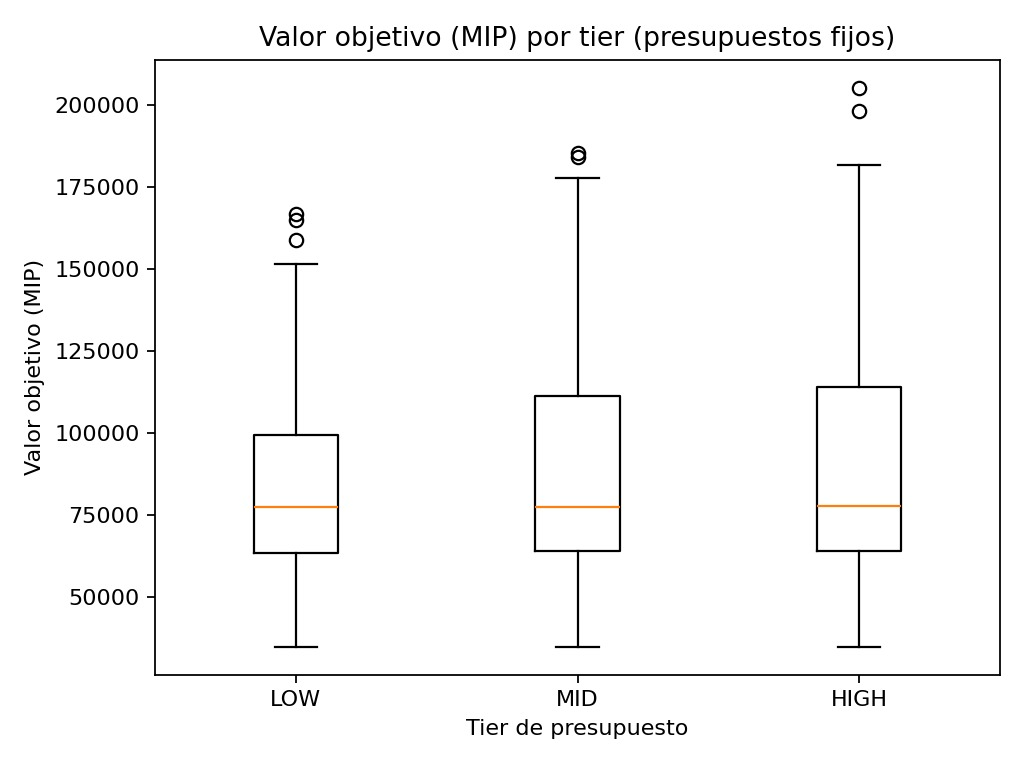
\includegraphics[width=0.5\textwidth]{figures/boxplotMIP.jpg}
	\caption[]{Gráfico muestra que medianas son parecidas entre tiers, pero la dispersion y los maximos crecen de low a mid a high.}
	\label{fig:boxplotMIP}
	\end{center}
\end{figure}

\begin{figure}[ht]
	\begin{center}
	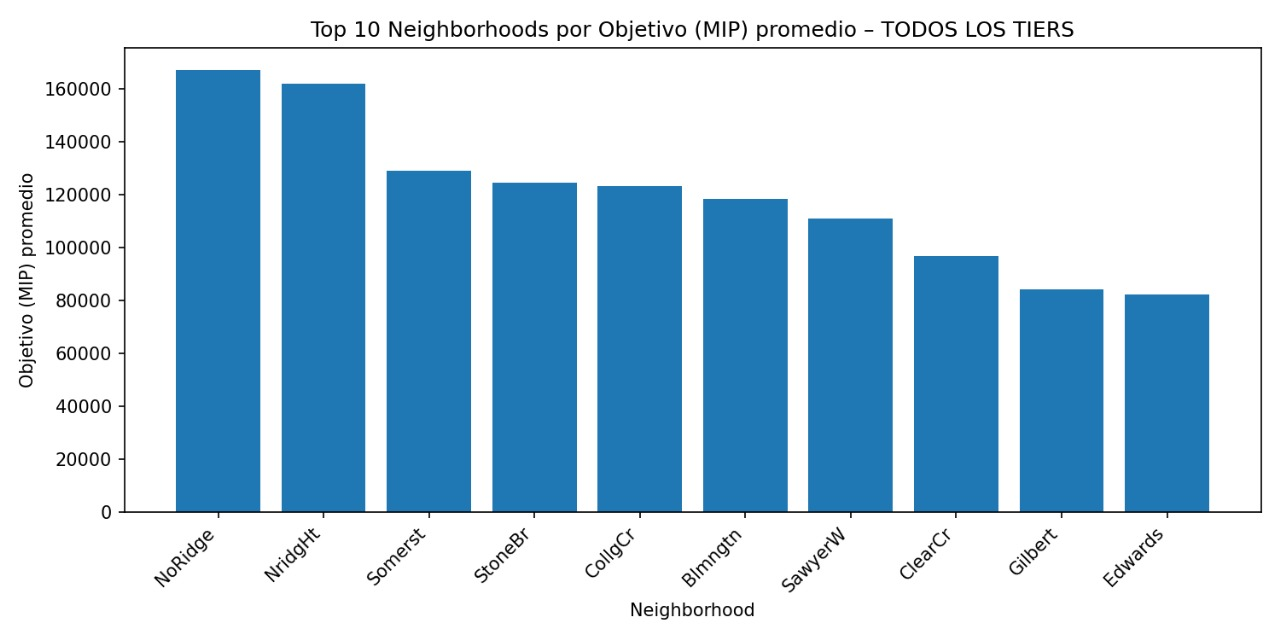
\includegraphics[width=0.5\textwidth]{figures/10 top neghborhoods.jpg}
	\caption[]{Gráfico muestra que medianas son parecidas entre tiers, pero la dispersion y los maximos crecen de low a mid a high.}
	\label{fig:top10NB}
	\end{center}
\end{figure}

\begin{figure}[ht]
	\begin{center}
	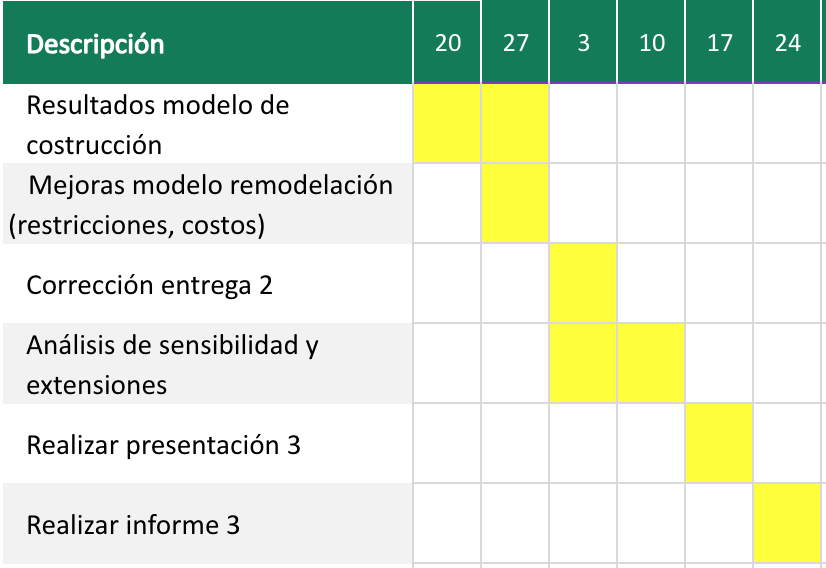
\includegraphics[width=0.5\textwidth]{figures/cartagantt.png}
	\caption[Carta Gantt]{Carta Gantt}
	\label{fig:CartaGantt}
	\end{center}
\end{figure}